\documentclass[sigconf]{acmart}
\AtBeginDocument{%
  \providecommand\BibTeX{{%
    Bib\TeX}}}

\usepackage{booktabs}
\usepackage{multirow}
\usepackage{pgfplots}
\pgfplotsset{compat=1.17}

\setcopyright{acmlicensed}
\copyrightyear{2026}
\acmYear{2026}
\acmDOI{}
\acmConference[CSE321]{Database Systems, Spring 2026}{}{UNIST}
\acmISBN{}

\settopmatter{printacmref=false}
\renewcommand\footnotetextcopyrightpermission[1]{}

\begin{document}

\title{CSE321 Project \#1: Implementation and Analysis of\\
B-tree, B*-tree, and B$^+$-tree Index Structures}

\author{Yongseong Eom (20211185)}
\affiliation{%
  \institution{UNIST}
  \country{South Korea}
}
\email{ekf3977@unist.ac.kr}

\renewcommand{\shortauthors}{Eom}

\maketitle

%==================================================================
\section{Problem Statement}
%==================================================================

Modern database systems use tree-based index structures to support
efficient point lookups, range scans, and updates over large datasets.
Three common variants are the B-tree, B*-tree, and B$^+$-tree, which
differ in where records are stored, how nodes are filled, and what
is done when a node overflows or underflows.

In this project I implement all three structures from scratch and
analyse them on a dataset of 100{,}000 student records. Each record
follows the schema
\texttt{(StudentID, Name, Gender, GPA, Height, Weight)}, where the
\texttt{StudentID} is used as the index key and the position of the
record in the in-memory array is used as the RID.

The code is written in JavaScript and runs on Node.js. No
third-party tree library is used. The fan-out parameter $d$ is
configurable and is interpreted as the \emph{minimum degree}, so
each node holds at most $2d-1$ keys and at most $2d$ children, and
every non-root node holds at least $d-1$ keys. The three trees use
the same $d$ and the same workload so that they can be compared
directly.

For grading, the public repository containing the source code,
dataset, and README is
\url{https://github.com/eom1202/cse321-project1}.

The required experiments are insertion (with $d \in \{3,5,10\}$),
point search, range query, and deletion.

%==================================================================
\section{Fundamental Index Structures: B-tree and B$^+$-tree}
%==================================================================

\subsection{B-tree}

Each node stores a sorted array of keys, an array of RIDs of the same
length, and an array of child pointers (empty if the node is a leaf).
Internal nodes therefore carry both keys and RIDs, so a search may
terminate as soon as the key is found, even at an internal node.

\paragraph{Search.} A standard recursive descent. The position of the
key inside a node is found by binary search; if not present and the
node is internal, the search continues in the matching child.

\paragraph{Insertion (top-down split).} Before moving down
into a child that is already full ($2d-1$ keys), the parent first
\emph{splits} that child. The median key of the full child is moved up
into the parent and the remaining keys are divided into two new nodes.
Because every child the algorithm visits has a free slot, the
recursion never has to back up.

\paragraph{Deletion.} While descending toward the key, the
algorithm makes sure the next child has at least $d$ keys: if it
does not, it either \emph{borrows} a key from a left or right
sibling through the parent, or, if both neighbours are already at
the minimum, \emph{merges} the child with a sibling and pulls a
separator down. Removing a key from an internal node replaces it
with its in-order predecessor or successor (whichever sub-tree has
spare capacity), or, if neither does, merges the two children and
recurses into the merged node.

\subsection{B$^+$-tree}

The B$^+$-tree uses the same fan-out ($2d-1$ keys per node) but a
different placement of records:

\begin{itemize}
\item Internal nodes store only keys and child pointers; they do
\textbf{not} hold RIDs.
\item All RIDs live in the leaves.
\item Every leaf has a \texttt{next} pointer to the leaf with the next
larger keys, forming a singly-linked list of leaves.
\item Search always descends to a leaf, even when the matching key
already appears as an internal separator.
\end{itemize}

\paragraph{Insertion.} Implemented bottom-up. The algorithm recurses
to the target leaf, inserts the key/RID, and then on the way back up
checks for overflow. Splitting a leaf \emph{copies} the smallest key
of the new right leaf into the parent as a separator and updates the
\texttt{next} pointers; splitting an internal node \emph{moves} the
middle key up.

\paragraph{Deletion.} A leaf underflows when it holds fewer
than $\lceil(2d-1)/2\rceil$ keys. The algorithm tries to borrow from
a sibling first and otherwise merges two leaves, taking care to relink
\texttt{next} pointers so that range scans remain consistent.
Internal-node underflow uses the same kind of borrow / merge rule,
with the parent separator used during rotation.

\paragraph{Range query.} The leaf chain makes range scans cheap:
locate the leaf containing the lower bound and follow \texttt{next}
pointers until a key exceeds the upper bound.

%==================================================================
\section{Advanced Index Structure: B*-tree}
%==================================================================

The B*-tree extends the B-tree by trying to keep nodes more full,
delaying splits as long as possible. When the algorithm encounters
a child that is already at $2d-1$ keys, the following decisions are
made in order:

\begin{enumerate}
\item \textbf{Redistribute} with a sibling if an adjacent sibling is
not full. The overflowing child, the sibling, and the parent
separator are pooled together and divided back into two nodes plus
one parent separator. If the overflow happens at a leaf, the new
key is added to the pool so that the insertion is finished in place;
if it happens at an internal node, the new key is not added because
it still has to move down into one of the rebalanced children. Either
way the split is avoided when the sibling has any free space.
\item \textbf{2-to-3 split} between the full child and an adjacent
full sibling. For a leaf split, the two full leaves, the parent
separator, and the new key are sorted together and then divided into
three nodes plus two new separators. For an internal-node split, the
two full children and the parent separator are divided into three
nodes, and insertion continues into the proper child.
\item As a last resort (only when the parent has a single child, in
particular when the root itself is the full node) a normal
1-to-2 split is performed.
\end{enumerate}

Search, range query, and deletion are inherited from the B-tree
implementation. The main difference is therefore the insertion
overflow policy. The implementation also tracks how often
redistribution and 2-to-3 split fire so that the experiment can
report them.

%==================================================================
\section{Experimental Results and Analysis}
%==================================================================

\subsection{Setup}

All experiments run on \texttt{student.csv} (100{,}000 records,
9-digit IDs of the form 2020XXXXX{--}2026XXXXX). Times are measured
with \texttt{performance.now()}. The 10{,}000 random search keys and
the 2{,}000 random deletion keys are drawn by a fixed-seed shuffle
so that all three trees see exactly the same workload.

The running times in the tables below come from a single
\texttt{node main.js student.csv} run. Individual times can vary
noticeably between runs, especially for the very fast operations
(point search and the 2{,}000-key deletion finish in a few
milliseconds, so a single GC pause or OS scheduling decision shifts
them by tens of percent). I therefore treat the time columns as
examples and base the analysis on the trend rather than the
exact value. The structural columns (splits, nodes, height,
utilization, matched count) are fixed and reproduce exactly
across runs.

\paragraph{Source code.}
The implementation and dataset are available at
\url{https://github.com/eom1202/cse321-project1}.
The \texttt{README.md} in that repository describes how to run the
experiments and the unit tests.

\subsection{Insertion and Parameter Tuning}

Table~\ref{tab:insert} reports the total insertion time for all
100{,}000 records, the fallback 1-to-2 split count, the final number
of nodes, the height of the tree, and the node utilization (total keys
divided by total node capacity).

\begin{table}[h]
\centering
\small
\caption{Insertion of 100{,}000 records.}
\label{tab:insert}
\begin{tabular}{cl rrrrr}
\toprule
$d$ & Tree & Time (ms) & Splits & Nodes & $h$ & Util.\\
\midrule
\multirow{3}{*}{3}
 & B-tree   &  75.8 & 31{,}365 & 31{,}374 & 9 & 63.7\,\% \\
 & B*-tree  & 135.1 &      7 & 24{,}615 & 8 & 81.3\,\% \\
 & B$^+$-tree &  64.6 & 34{,}977 & 34{,}985 & 8 & 72.6\,\% \\
\midrule
\multirow{3}{*}{5}
 & B-tree   &  49.0 & 16{,}591 & 16{,}597 & 6 & 66.9\,\% \\
 & B*-tree  &  78.5 &      5 & 13{,}149 & 6 & 84.5\,\% \\
 & B$^+$-tree &  35.5 & 17{,}939 & 17{,}945 & 6 & 71.5\,\% \\
\midrule
\multirow{3}{*}{10}
 & B-tree   &  42.4 &  7{,}709 &  7{,}714 & 5 & 68.2\,\% \\
 & B*-tree  &  63.1 &      3 &  6{,}100 & 4 & 86.3\,\% \\
 & B$^+$-tree &  26.6 &  8{,}072 &  8{,}077 & 5 & 70.1\,\% \\
\bottomrule
\end{tabular}
\end{table}

For the B*-tree, the split count in Table~\ref{tab:insert} reports
only fallback 1-to-2 splits. Most overflows are absorbed by the
redistribute and 2-to-3 paths instead. The actual breakdown is shown
in Table~\ref{tab:bstar}.

\begin{table}[h]
\centering
\small
\caption{B*-tree: how each overflow was resolved.}
\label{tab:bstar}
\begin{tabular}{c rrr}
\toprule
$d$ & Redistribute & 2-to-3 split & 1-to-2 split \\
\midrule
3  & 57{,}136 & 24{,}600 & 7 \\
5  & 46{,}209 & 13{,}138 & 5 \\
10 & 33{,}559 &  6{,}093 & 3 \\
\bottomrule
\end{tabular}
\end{table}

\paragraph{Discussion.} Larger $d$ reduces tree height and node count
for every tree. The B$^+$-tree has simple insertion logic because data
records only live in leaves, and it performs well on this workload.
The B*-tree does extra work before splitting, so insertion takes more
work, but it uses much fewer nodes. At $d=10$ it
stores the same 100{,}000 keys in 6{,}100 nodes (utilization
$86.3\,\%$), while the B-tree uses 7{,}714 nodes (utilization
$68.2\,\%$). This shows the main purpose of B*-tree redistribution:
spend more insertion time to keep pages more full.

Figure~\ref{fig:util} shows utilization vs.\ $d$ for the three trees.

\begin{figure}[h]
\centering
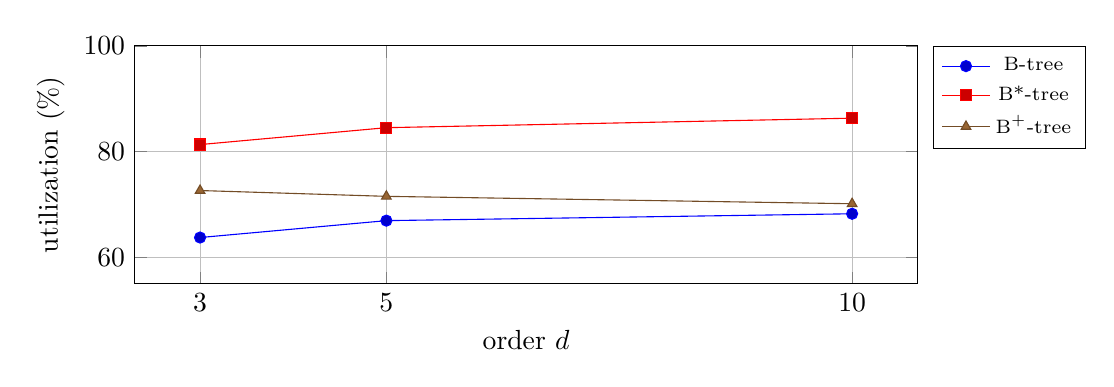
\begin{tikzpicture}
\begin{axis}[
  width=0.95\linewidth, height=4.6cm,
  xlabel={order $d$}, ylabel={utilization (\%)},
  xtick={3,5,10}, ymin=55, ymax=100,
  legend style={font=\scriptsize, at={(1.02,1)}, anchor=north west},
  grid=both,
]
\addplot+[mark=*]   coordinates {(3,63.7) (5,66.9) (10,68.2)};
\addplot+[mark=square*] coordinates {(3,81.3) (5,84.5) (10,86.3)};
\addplot+[mark=triangle*] coordinates {(3,72.6) (5,71.5) (10,70.1)};
\legend{B-tree, B*-tree, B$^+$-tree}
\end{axis}
\end{tikzpicture}
\caption{Node utilization after inserting 100{,}000 records.}
\label{fig:util}
\end{figure}

\subsection{Point Search}

10{,}000 random Student IDs were drawn from the dataset and looked up
in each tree. Table~\ref{tab:search} reports the total time and the
mean per query.

\begin{table}[h]
\centering
\small
\caption{Point search of 10{,}000 random keys.}
\label{tab:search}
\begin{tabular}{cl rr}
\toprule
$d$ & Tree & Total (ms) & Mean ($\mu$s/q)\\
\midrule
\multirow{3}{*}{3}
 & B-tree   & 6.21 & 0.62 \\
 & B*-tree  & 6.12 & 0.61 \\
 & B$^+$-tree & 7.92 & 0.79 \\
\midrule
\multirow{3}{*}{5}
 & B-tree   & 5.06 & 0.51 \\
 & B*-tree  & 3.75 & 0.38 \\
 & B$^+$-tree & 4.79 & 0.48 \\
\midrule
\multirow{3}{*}{10}
 & B-tree   & 2.46 & 0.25 \\
 & B*-tree  & 3.30 & 0.33 \\
 & B$^+$-tree & 2.96 & 0.30 \\
\bottomrule
\end{tabular}
\end{table}

\paragraph{Discussion.} Point search is very fast for all three
trees, so small timing differences are not very stable. The B*-tree
performs well for $d=3$ and $d=5$ in this run, mainly because it has
fewer nodes (and at $d=3$ a smaller height as well). At $d=10$, the
three trees are close enough that the ordering can change between
runs. Both the B-tree and the B*-tree allow the search to stop at an
internal node, but the B*-tree's nodes are denser, so each level does
slightly more comparison work. With heights so close together, this
extra work per level can offset the height advantage. The B$^+$-tree
always descends to a leaf, but its internal nodes are compact. Also,
when the whole dataset is in memory, cache and JavaScript runtime
effects can be larger than the theoretical difference.

\subsection{Range Query}

The range query follows the example in the project manual: the
average GPA and average height of \emph{male} students whose ID lies
in $[202{,}000{,}000, 202{,}100{,}000]$. The PDF example uses
8-digit IDs ($20{,}200{,}000$--$20{,}210{,}000$); the dataset uses
9-digit IDs of the form $2020\text{xxxxx}\dots 2026\text{xxxxx}$, so
I use the matching 9-digit range. The query matches 7{,}215
students with average GPA $3.278$ and average height $174.06$ cm in
all three trees, which is a useful correctness check.

\begin{table}[h]
\centering
\small
\caption{Range query (matched 7{,}215 male records).}
\label{tab:range}
\begin{tabular}{c rrr}
\toprule
$d$ & B-tree & B*-tree & B$^+$-tree \\
\midrule
3  & 3.76 ms & 3.14 ms & 3.93 ms \\
5  & 2.57 ms & 1.60 ms & 1.39 ms \\
10 & 0.97 ms & 0.92 ms & 0.79 ms \\
\bottomrule
\end{tabular}
\end{table}

\paragraph{Discussion.} The B$^+$-tree is designed for range scans
because its leaves are linked. In this workload it is competitive with
the B*-tree, whose smaller node count also helps range traversal touch
less structure. The B-tree is less specialized for this query because
it has neither advantage: no leaf-linked list to stream through, and
no compact node count from the redistribute policy.

\subsection{Deletion and Structural Integrity}

2{,}000 random keys were removed from each tree, after which the
deletion time was measured. Table~\ref{tab:delete} also reports the
state of each tree after deletion (node count, height, utilization).

\begin{table}[h]
\centering
\small
\caption{Deletion of 2{,}000 random keys.}
\label{tab:delete}
\begin{tabular}{cl rrrr}
\toprule
$d$ & Tree & Time (ms) & Nodes & $h$ & Util. \\
\midrule
\multirow{3}{*}{3}
 & B-tree   & 4.25 & 30{,}867 & 8 & 63.5\,\% \\
 & B*-tree  & 2.03 & 24{,}614 & 8 & 79.6\,\% \\
 & B$^+$-tree & 2.90 & 34{,}618 & 8 & 72.0\,\% \\
\midrule
\multirow{3}{*}{5}
 & B-tree   & 1.57 & 16{,}505 & 6 & 66.0\,\% \\
 & B*-tree  & 1.07 & 13{,}149 & 6 & 82.8\,\% \\
 & B$^+$-tree & 1.73 & 17{,}834 & 6 & 70.6\,\% \\
\midrule
\multirow{3}{*}{10}
 & B-tree   & 1.15 &  7{,}704 & 5 & 67.0\,\% \\
 & B*-tree  & 1.05 &  6{,}100 & 4 & 84.6\,\% \\
 & B$^+$-tree & 1.15 &  8{,}041 & 5 & 69.0\,\% \\
\bottomrule
\end{tabular}
\end{table}

\paragraph{Discussion.} All three trees deleted exactly the 2{,}000
target keys and kept the remaining keys searchable. The B*-tree keeps
the highest utilization after deletion because its nodes were already
more full after insertion. The deletion implementation itself follows
the B-tree borrow/merge policy, so any B*-tree timing advantage mostly
comes from the smaller tree created during insertion. The absolute
times are small, so the exact ordering should not be read too strongly.

%==================================================================
\section{Summary}
%==================================================================

I implemented and compared three classical index structures over a
100{,}000-record dataset.

\begin{itemize}
\item The \textbf{B-tree} is the simplest of the three. It stores RIDs
in internal nodes and leaves, so point search can sometimes stop
early. Its weakness is low node utilization (about $63$--$68\,\%$).
\item The \textbf{B*-tree} keeps nodes the most full (up to
$86.3\,\%$ at $d=10$) because redistribute and 2-to-3 split absorb
almost all overflows. The price is extra insertion work.
\item The \textbf{B$^+$-tree} has simple insertion logic in this
implementation, and its leaf-linked list is useful for range queries.
Its point search always reaches a leaf.
\end{itemize}

In short: the B-tree is the simplest baseline, the B*-tree is the
most space-efficient, and the B$^+$-tree is the easiest to scan in
order. Each is the right answer to a different question.

%\bibliographystyle{ACM-Reference-Format}
%\bibliography{reference}

\end{document}
